\section{Results}
In tables \ref{aha-table:graphsize} and \ref{aha-table:searcheffort} we evaluate the performance of AHA* in terms of several variables. 
Firstly, we look at the effect of increasing the amount of soft obstacles (SO) from 0\% (the original test maps with only one traversable terrain) to 5\% and 10\% respectively. 
We also contrast high and low quality abstractions (denoted HQ and LQ) on a range of cluster sizes $\lbrace 10, 15, 20 \rbrace$ (denoted CS10, CS15 and CS20).
\par \indent
In table \ref{aha-table:graphsize} we present the average size of the abstract graph in nodes and edges relative to the size of the original graphs which featured an average 4469 nodes and 16420 edges. 
\input gsntable.tex
As expected, the number of both nodes and edges decreases as cluster size increases on each set of test maps. Interestingly, there is a 2-3 fold increase in the number of edges as we move from SO 0\% to SO 5\%; this reflects the increasing complexity of terrain in each cluster and confirms the predictions of lemmas \ref{aha-lemma:maxedgesincluster} and \ref{aha-lemma:maxtransitions} which also hold moving from 5\% SO to 10\% SO (though the increase is less dramatic). 
\par \indent
Perhaps most interesting is the counter-balancing effect on graph size stemming from the quality of the abstraction; there is approximately a 5-fold decrease in the number of edges and 2-3 fold reduction in nodes going from a HQ graph to a LQ approximation.
The best cases appear to be associated with larger cluster sizes which is expected. 
Even in the worst observed case however the LQ graph has just 6.7\% the number of edges in the original grid and only 4.8\% nodes. 
If we assume each non-abstract node and edge require one byte of memory to store, then our abstract graph, which contains 2 annotations per edge (capability and clearance, each requiring 1 byte), will still have a space complexity less than 20\% of the original graph even using a naive implementation. 
Custom implementations could reduce this further still although the most significant gains appear to come from simply increasing the cluster size; in this case, going from CS10 to CS20 almost halves the memory required to store the set of abstract edges.
\par \indent
Next we consider the performance of AHA* with respect to path quality. We measure this as:
$$ \%error = \frac{apl - opl}{opl} \times 100 $$ where $opl$ is the length of the optimal path as calculated by AA* and $apl$ the length of the abstract path used by AHA*.
Figure \ref{aha-fig:allgraphs}(top) shows the average performance of HQ and LQ abstractions with respect to each cluster size. 
\begin{figure}[htbp]
       \caption{\small{\emph{AHA* performance (HQ vs LQ abstraction). Top: Path quality. Bottom: Search effort. }}}
       \begin{center}
                       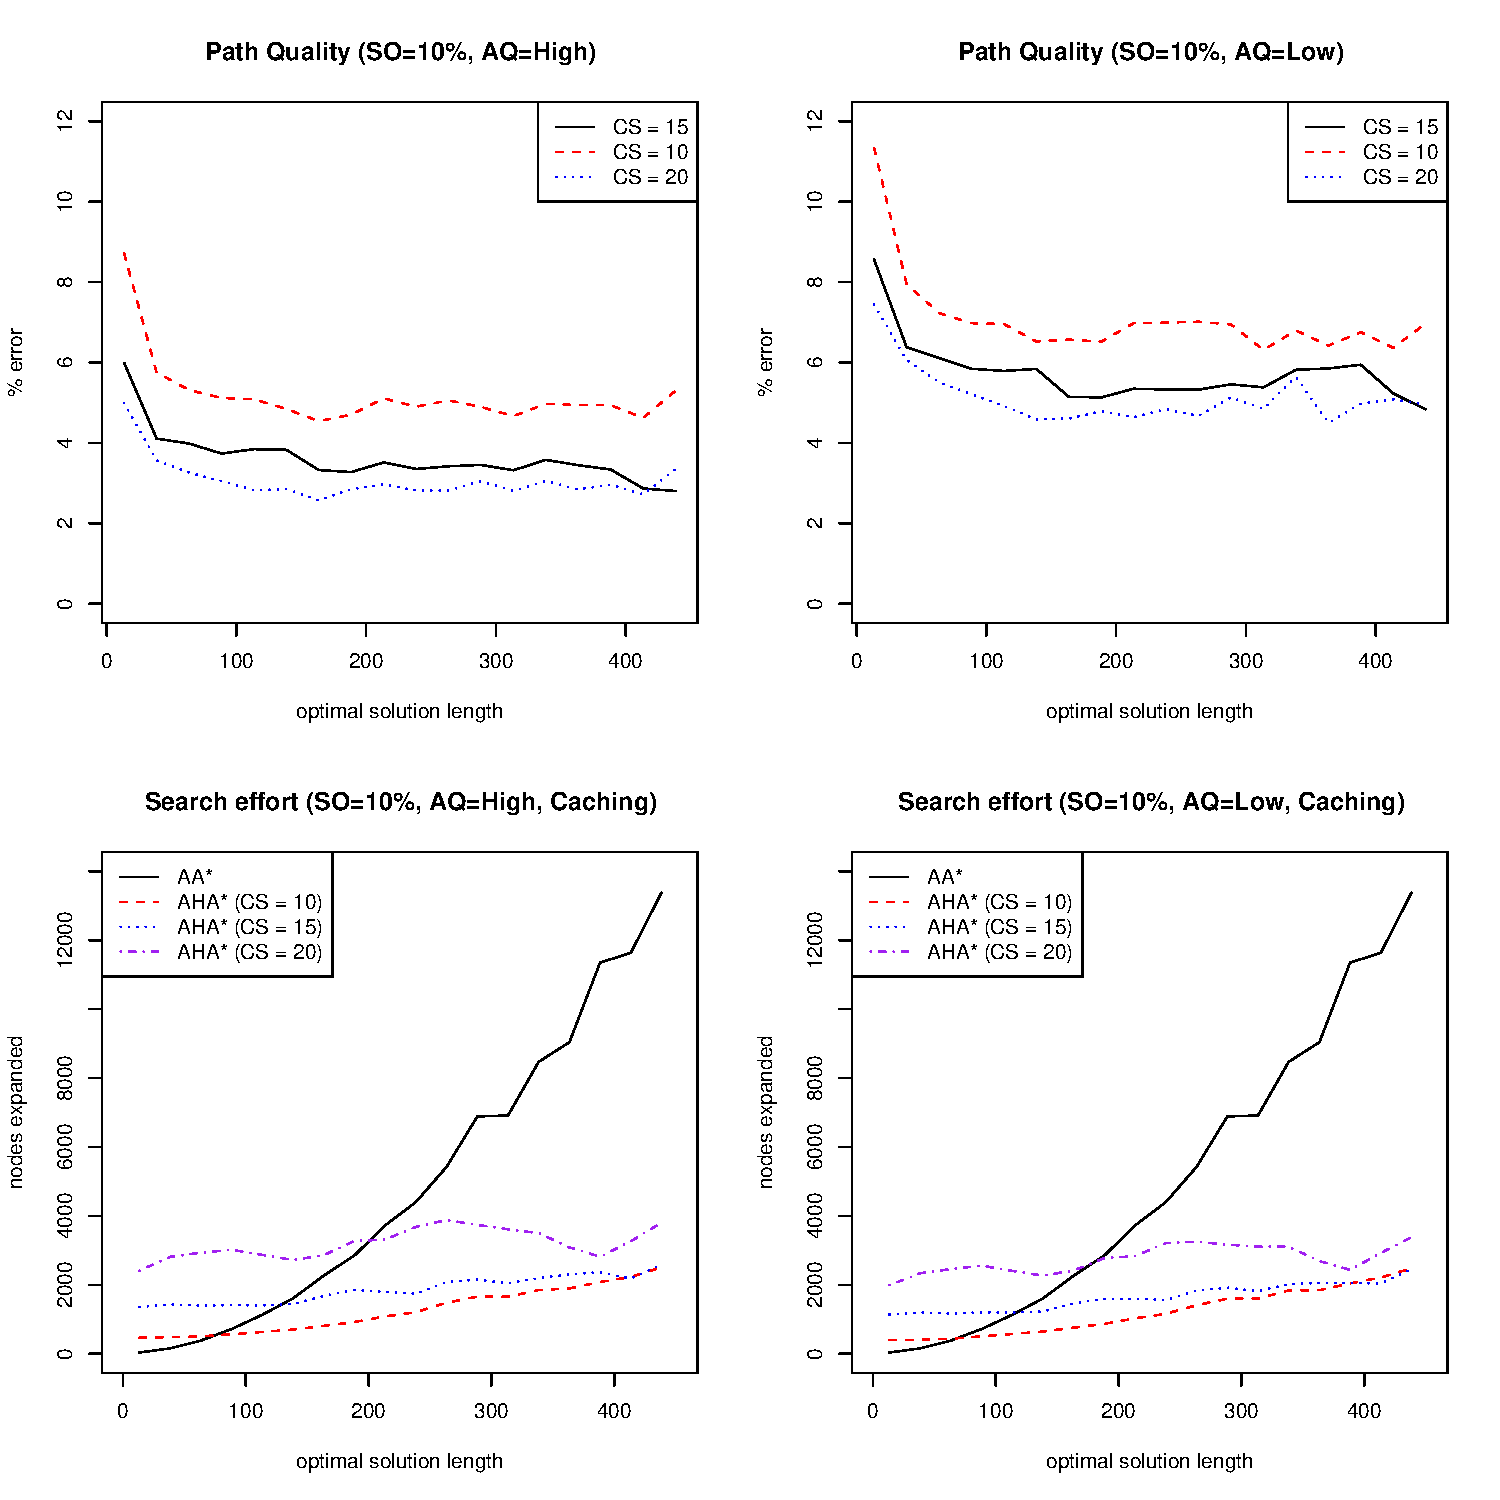
\includegraphics[scale=0.35]{diagrams/allgraphs.pdf}
       \end{center}
       \label{aha-fig:allgraphs}
\end{figure}
Overall, using HQ abstraction yields a very low error for the test, between 3-5\%. 
Perhaps most encouraging however are the results for LQ abstractions. 
Despite the 5-fold reduction in the number of edges, on average, AHA* still performs in the 7-10\% range, giving up relatively little optimality. 
This provides strong support for theorem \ref{aha-theorem:weakdominance} and the intuition behind it; roads can take an agent to most of the same places dirt roads and trails can without too much detour.
The higher than average error observed for short paths is due to AHA*'s inability to find a direct route from start to goal -- unlike AA*.
As the length of the problem increases this localised error becomes less an issue.
\par \indent
A more complete picture of AHA*'s path quality performance is given in table \ref{aha-table:pathquality} where we observe similar trends. 
\input pqtable.tex
A quick glance confirms initial expectations; bigger clusters result in better performance. 
In some cases however (0\%SO and 5\% SO) going from CS15 HQ/LQ to CS20 HQ/LQ produces a marginal decrease in quality. 
This seemingly counter-intuitive result can be explained by our inter-edge placement strategy. 
In all situations the pair of nodes with maximal clearance in an entrance tends to be towards the beginning of the entrance which is not an optimal placement. 
On maps that produce low-complexity clusters of predominately one terrain we identify fewer entrances and there are fewer transition points between clusters. 
\cite{botea04} address this issue by placing multiple transition points per entrance whereas we choose only one. 
The biggest increase in path quality is thus observed as we move toward more complex maps which generate more transitions. 
Table \ref{aha-table:pathquality} confirms this; for the SO 10\% set of maps the problem dissapears. 
It appears AHA* is so optimised for complex cases that it suffers some minor performance degredation on simpler problems. 
\par \indent
Finally, we turn our attention to figure \ref{aha-fig:allgraphs}(bottom) where we evaluate AHA* using a search effort metric. 
\input setable.tex
We contrast the total number of nodes expanded by AHA* (insertion + hierarchical search + refinement) with AA*.
A more complete set of results is given in table \ref{aha-table:searcheffort} where we contrast total effort with insertion effort; the latter is presented as a \% of the total.
\par \indent
We observe that the set of experiments using large clusters are disadvantaged in this test. 
The insertion effort required to connect start and goal to each abstract node in their local clusters heavily dominates the total effort and AHA* CS20 even trails AA* for problems up to length 250. 
We can see the gap between CS20 and the smaller cluster sizes decrease as problem size grows but our benchmark set of experiments are not hard enough for such coarse-grain map decompositions to be advantageous. 
The difference is less pronounced using LQ graphs (there are less abstract nodes per cluster) however it appears CS10 or CS15 are more suitable choices for problems up to our maximum length, 450.
